\subsection{方法2}
运行给的示例程序3.2就找到了0001 -> 0001 -> 0001 -> 0001 -> 0001这条路线

这条路线就是全局下的最优解不假，但是给的示例程序问题就是只找到了这么一条路线

不过还有可能有与他概率相等的另一条路线

一开始思路是，每一轮多保存几个差分，最后笛卡尔积，串起来，但那样好像挺麻烦，

当我盯着示例程序的时候，有了一个想法

我们这里把输入差分为0的初始概率设成0，就是因为它必然以概率为1得到输出差分为0，所以你如果把这个也设成1

那么最后找到的最优路线肯定是全0
\begin{figure}[H]
    \centering
    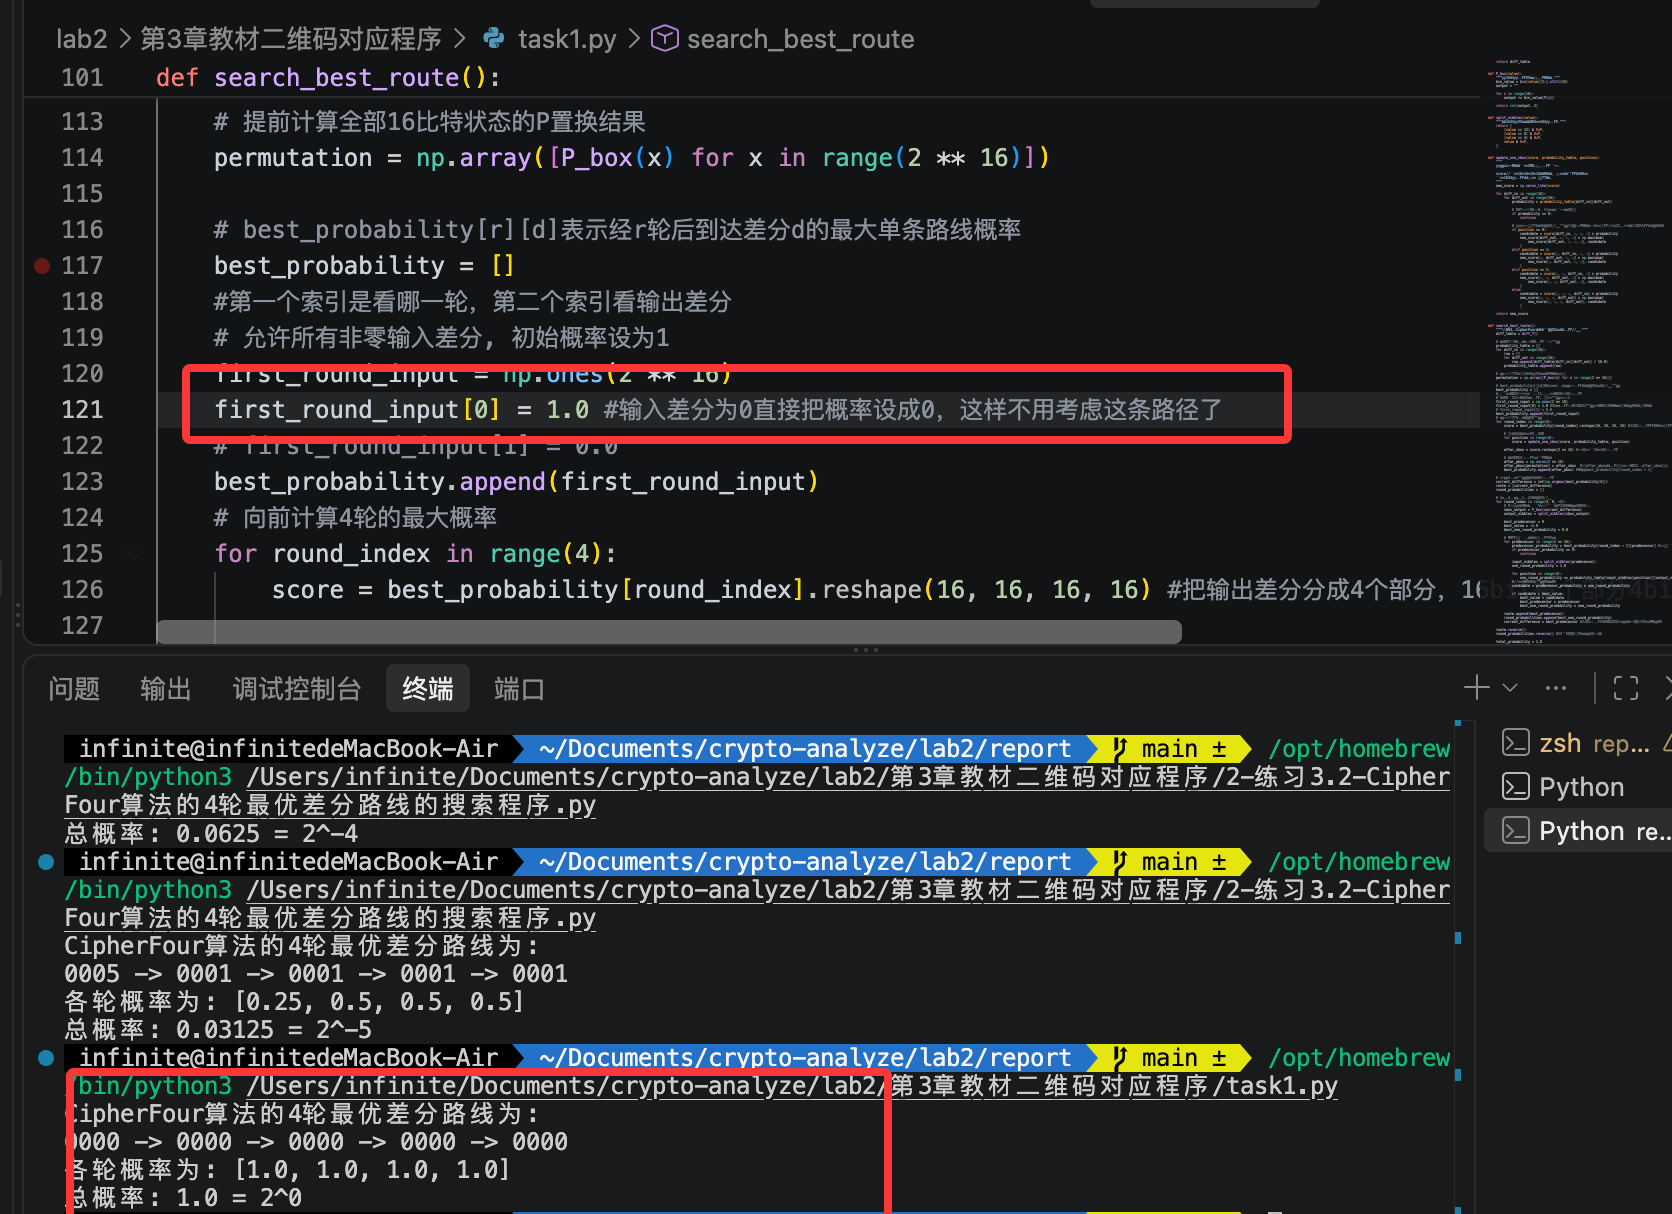
\includegraphics[width=0.8\textwidth]{figures/test1.png}
    \caption{概率设成1}
\end{figure}

换而言之，初始概率为0就能屏蔽这条路线，前面就是通过把输入为0排除掉，从而得到了0001这条路线

那我如果要找另一条路线，再把0001屏蔽掉，不就好了吗？

两个路线相同，肯定是每一步都相同，那说句废话，两个路线不同，自然就是有一步不同就行

所以我们每一轮都尝试屏蔽0001，然后找其中概率最大的，就是题目要求的不同于0001这条路线的最好情况了
\subsection{第一轮不同}
\begin{figure}[H]
    \centering
    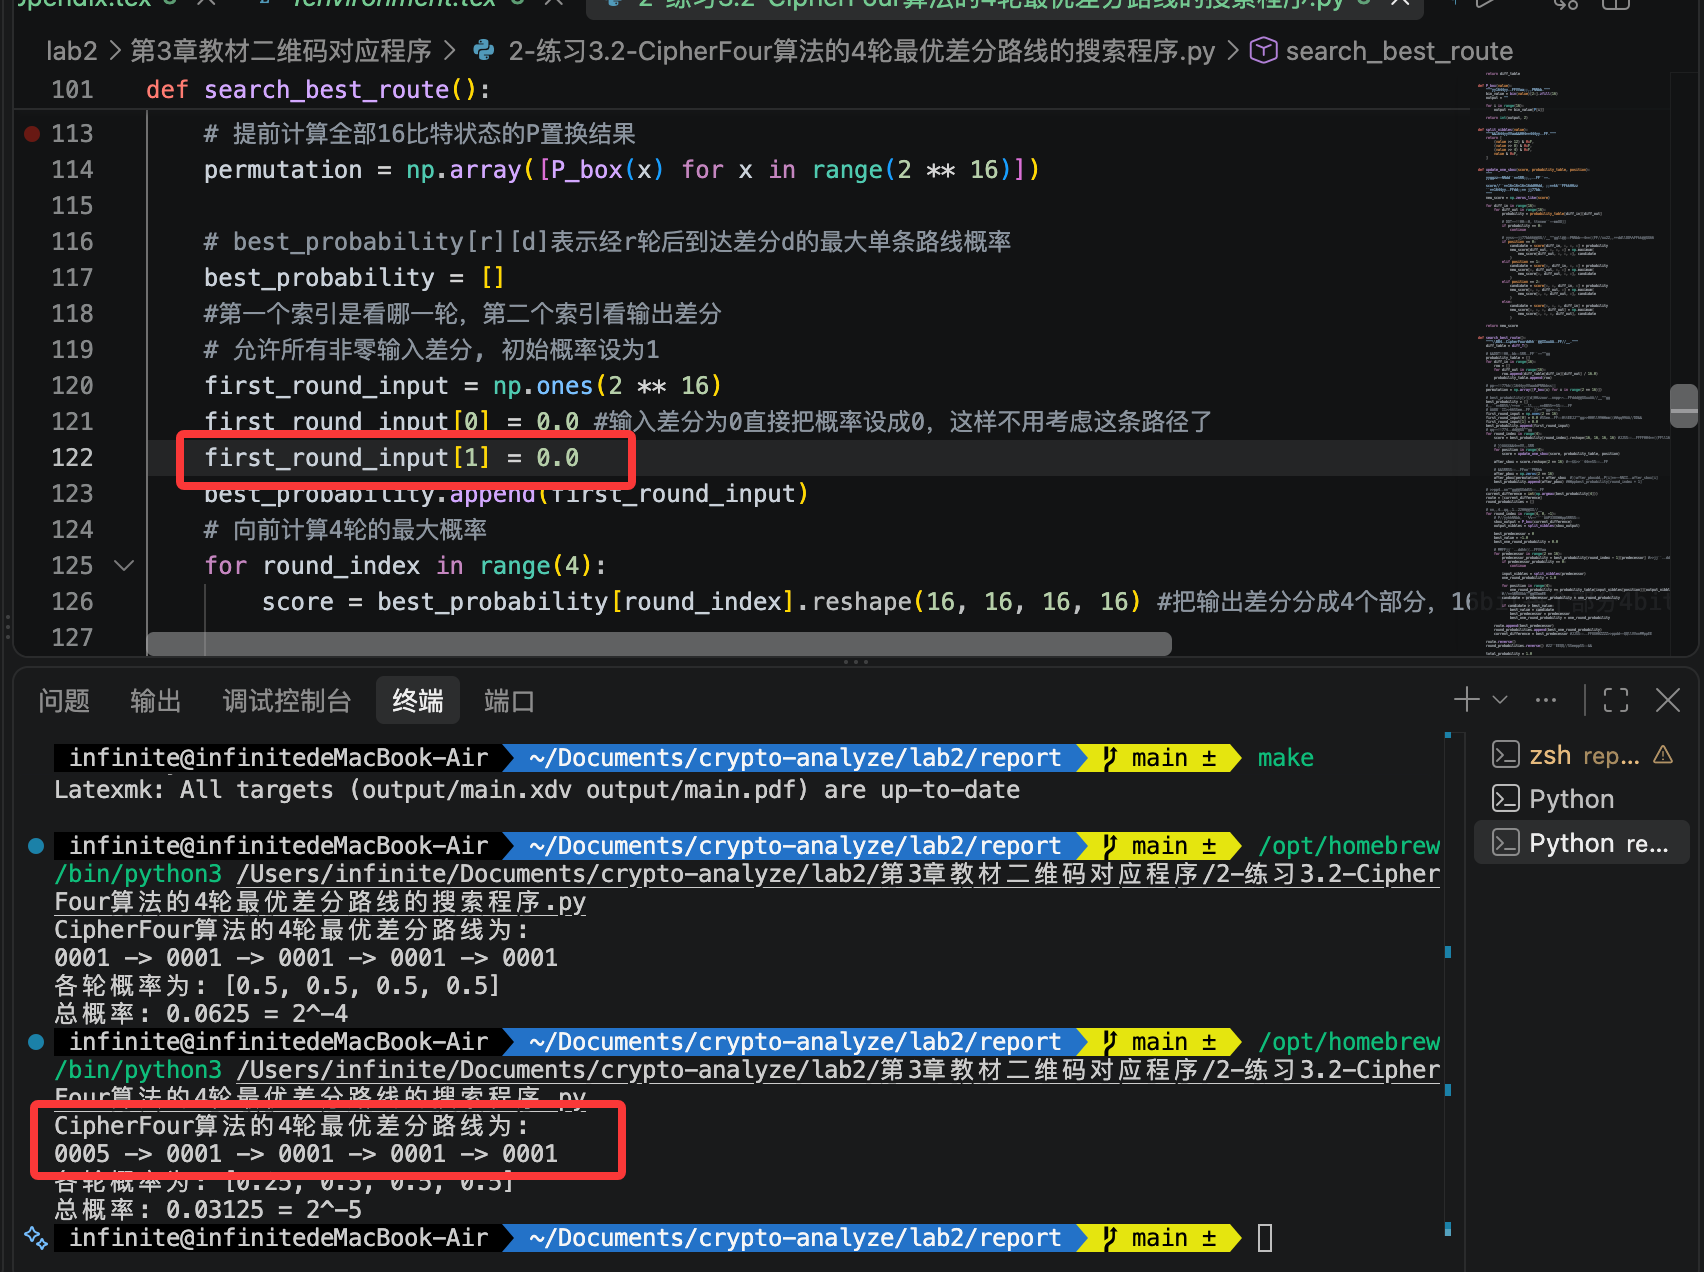
\includegraphics[width=0.8\textwidth]{figures/find1.png}
    \caption{初始禁用0001}
\end{figure}
可以看到找到了0005 -> 0001 -> 0001 -> 0001 -> 0001这条路线

这个不好
\subsection{找到其他路线}
嗯，很多时候有了开始，后面就很简单了，我们每个位置都禁用一下，给search\_best\_route加个pos参数，分别禁用每一次
\begin{figure}[H]
    \centering
    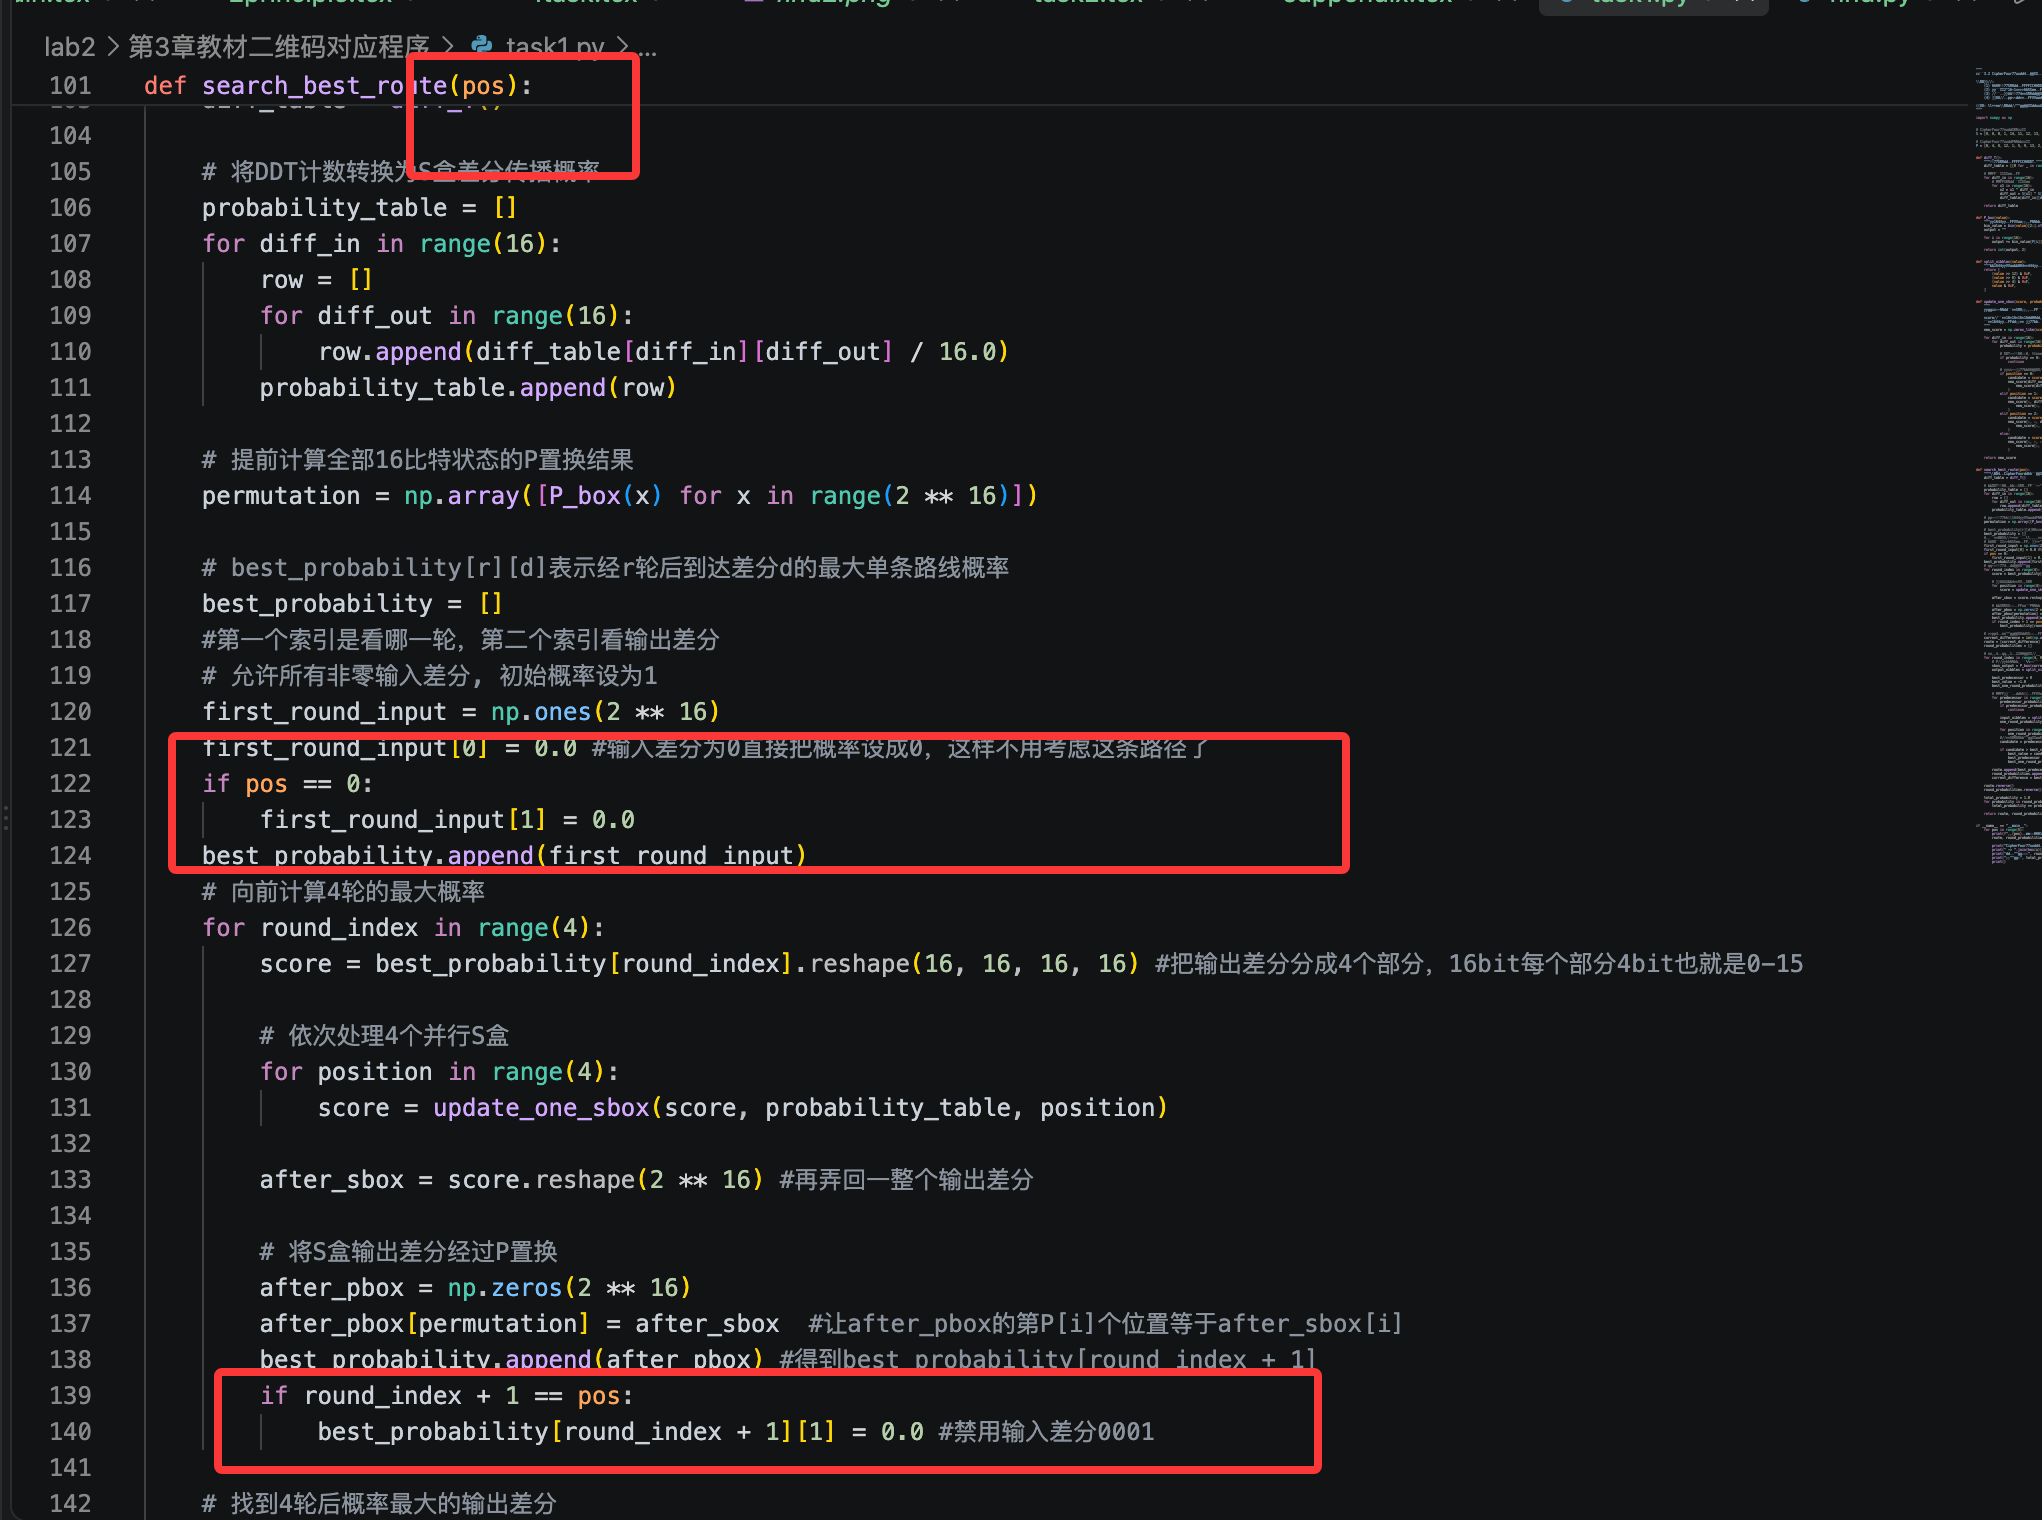
\includegraphics[width=0.8\textwidth]{figures/task1_enhance.png}
    \caption{修改代码}
\end{figure}

遗憾的是，没有和前面给的概率相等的路线，最多只有概率为1/32的了
\begin{figure}[H]
    \centering
    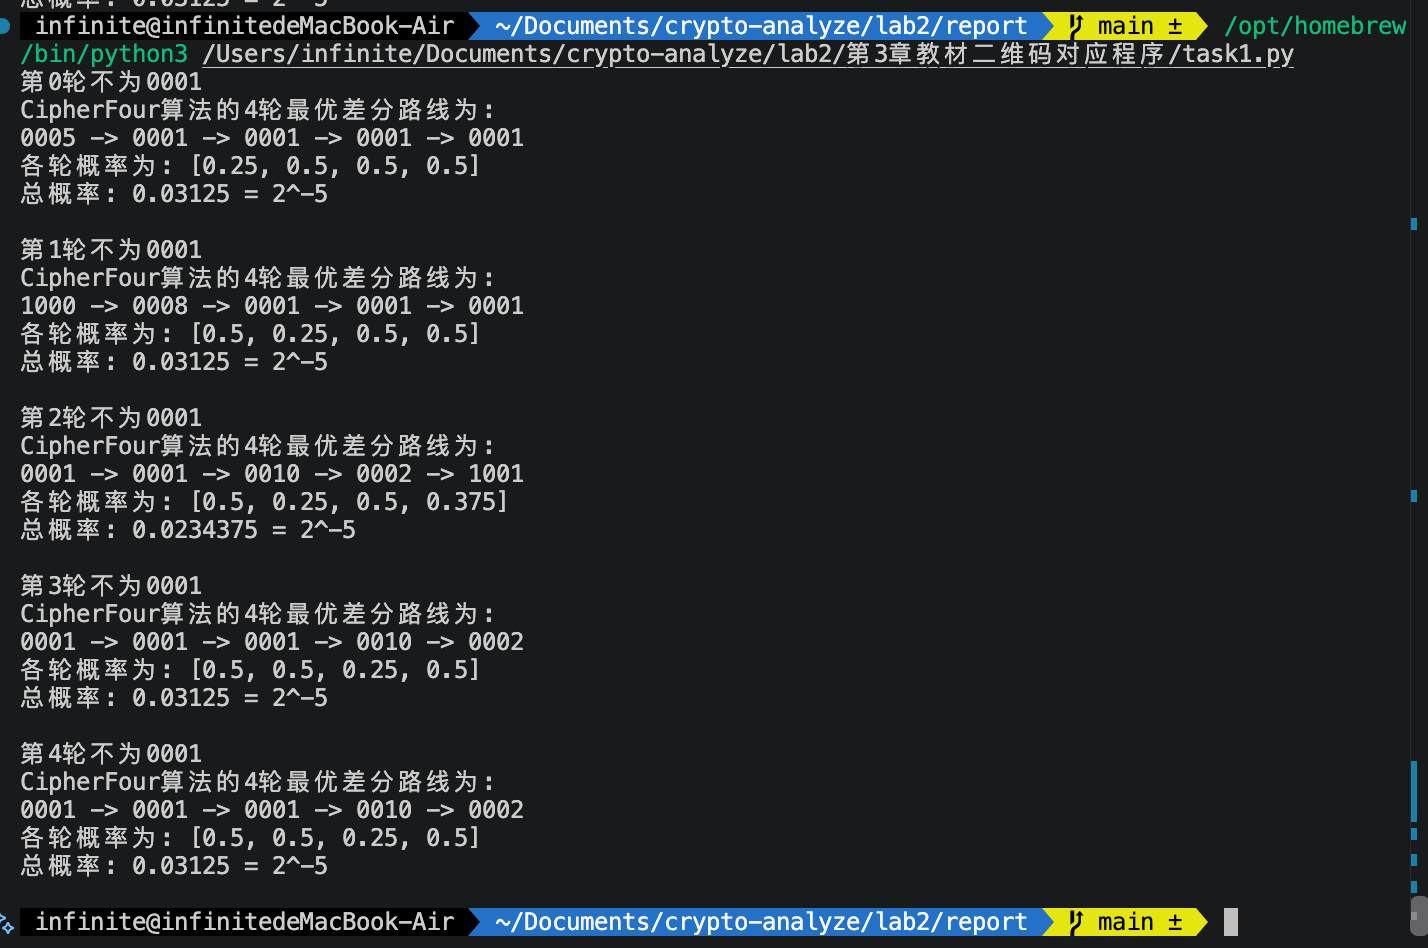
\includegraphics[width=0.8\textwidth]{figures/task1_result.png}
    \caption{结果}
\end{figure}

找到了五条路线，概率都一样，不过题目要求只看\(\Delta_{\text{in}} \rightarrow \Delta_{\text{out}}\)

那么其实就是四条

0005->0001

1000->0001

0001->1001

0001->0002
